\clearpage

\section{Theoretical Analysis}
\label{sec:analysis}

In this part we will discuss the theoretical analysis of the circuit shown in \ref{}.

%\begin{multicols}{2}
%
%  \begin{figure}[H]
%  \begin{center}
%   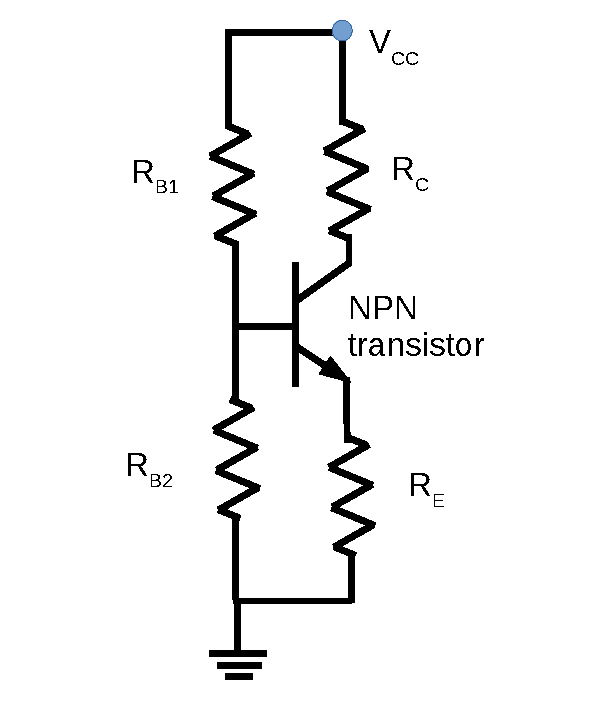
\includegraphics[width=6cm]{lab4_DC1.pdf}
%  \caption{Gain stage OP computation.}
%  \label{fig:DC analysis}
%  \end{center}
%  \end{figure}
%  
%  
%  \begin{figure}[H]
%  \begin{center}
%   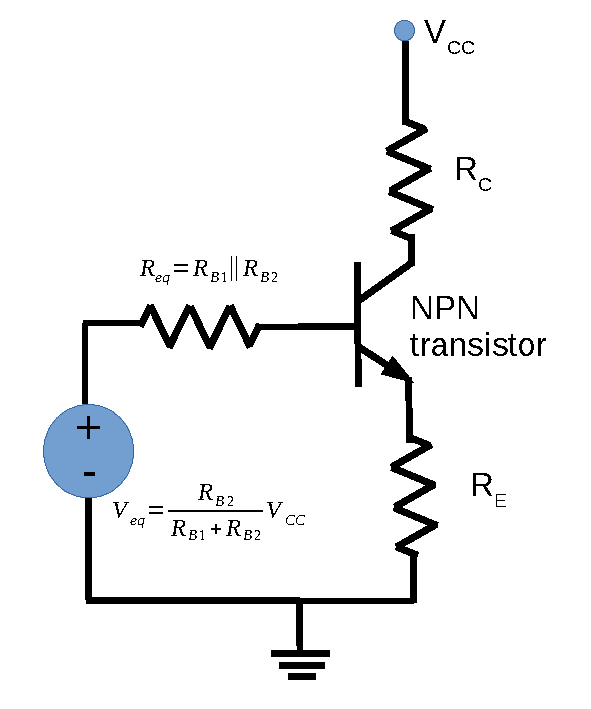
\includegraphics[width=6cm]{lab4_DC1_TH.pdf}
%  \caption{Thévenin equivalent.}
%  \label{fig:Thevenin}
%  \end{center}
%  \end{figure}
%\end{multicols}

%\begin{table}[h]
%    \centering
%    \begin{tabular}{|l|r|}
%      \hline
%      {\bf Name} & {\bf Value [A or V]} \\ \hline
%      \input{../mat/op1_tab.tex}
%    \end{tabular}
%    \caption{Current through collector and the voltage drop between collector and emitter.}
%    \label{tab:op1_tab}
%  \end{table}

%\begin{figure}[H]
%  \begin{center}
%   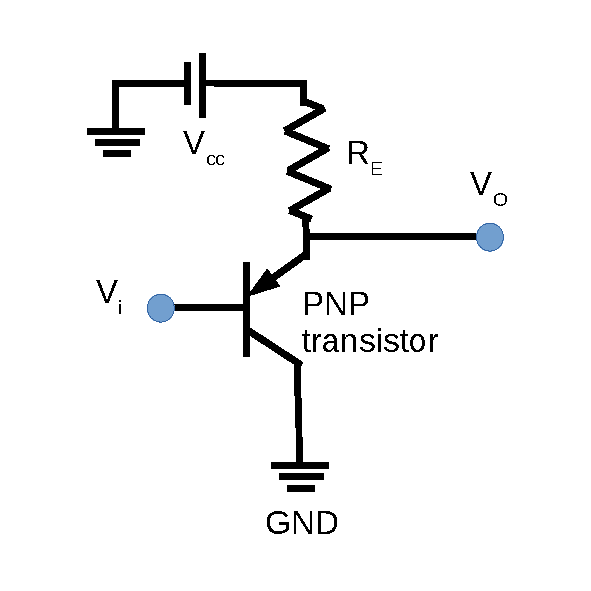
\includegraphics[width=10cm]{lab4_DC2.pdf}
%  \caption{Output stage (DC analysis).}
%  \label{fig:Thevenin2}
%  \end{center}
%  \end{figure}.

As one may notice, there are a few differences when comparing \textit{Ngspice}'s and \textit{Octave}'s results.
But this is somewhat normal since the models used in the theoretical analysis are approximations of non linear components that are the transistors.
Moreover, the Hybrid $\Pi$ model used was not the full one, so we did not take into account the Miller effect and complete Early Effect
that occurs in this type of network. Despite this, the results are quite satisfactory.
